\documentclass[12pt, varwidth, border=5mm]{standalone}
\usepackage{tikz}
\usepackage{amsmath}
% Underlining package
\usepackage{ulem}
\usetikzlibrary{calc}
\usetikzlibrary{angles,quotes}
% \usepackage[a4paper, portrait, margin=1cm]{geometry}

\begin{document}
\section*{ }
    \begin{minipage}{0.55\textwidth}
  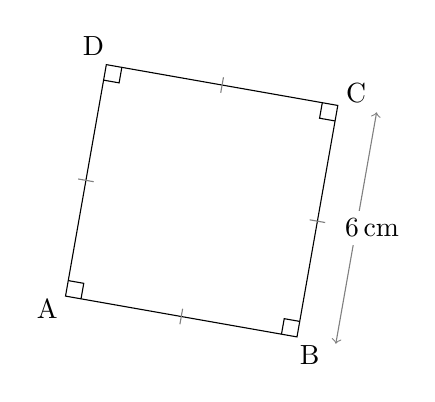
\begin{tikzpicture}[scale=1.0, baseline=(current bounding box.north)]
    \begin{scope}[rotate=-10]
        % Draw square
        \draw (0,0) coordinate (A) --
              ++(2.985,0) coordinate (B) --
              ++(0,2.985) coordinate (C) --
              ++(-2.985,0) coordinate (D) -- cycle;

        % Right angle markers
        \foreach \p/\q/\r in {D/A/B,A/B/C,B/C/D,C/D/A} {
            \pic [draw, -, angle radius=0.2cm] {right angle=\p--\q--\r};
        }

        % Vertex LABELS
        % Labels relative to shape geometry
        \node at ($(A)+(-0.2,-0.2)$) {A};
        \node at ($(B)+(0.2,-0.2)$) {B};
        \node at ($(C)+(0.2,0.2)$) {C};
        \node at ($(D)+(-0.2,0.2)$) {D};

        % Tick marks across horizontal sides
        \draw[thin, gray]
            ($(A)!0.5!(B) + (0,-0.10)$) --
            ($(A)!0.5!(B) + (0,0.10)$);

        \draw[thin, gray]
            ($(D)!0.5!(C) + (0,-0.10)$) --
            ($(D)!0.5!(C) + (0,0.10)$);

        % Tick marks across vertical sides
        \draw[thin, gray]
            ($(B)!0.5!(C) + (-0.10,0)$) --
            ($(B)!0.5!(C) + (0.10,0)$);

        \draw[thin, gray]
            ($(A)!0.5!(D) + (-0.10,0)$) --
            ($(A)!0.5!(D) + (0.10,0)$);

        % dotted/dashed arrows shifted away from edges
        % % Vertical side (B-C), shifted right
        \draw[<->, gray]
            ($(B) + (0.50cm,0)$) -- ($(C) + (0.50cm,0)$)
            node[black, midway, fill=white, xshift=2mm, inner sep=3pt] {6\,cm};

    \end{scope}
\end{tikzpicture}
\end{minipage}%
\hfill
\begin{minipage}{.4\textwidth}
  \begin{align*}
  \text{Area} &= l^2 \\
  \text{Area} &= 6 \,\text{cm} \times 6 \,\text{cm} \\
  \text{Area} &= 36 \,\text{cm}^2
  \end{align*}
\end{minipage}

\end{document}
